% mnras_template.tex 
%
% LaTeX template for creating an MNRAS paper
%
% v3.0 released 14 May 2015
% (version numbers match those of mnras.cls)
%
% Copyright (C) Royal Astronomical Society 2015
% Authors:
% Keith T. Smith (Royal Astronomical Society)

% Change log
%
% v3.0 May 2015
%    Renamed to match the new package name
%    Version number matches mnras.cls
%    A few minor tweaks to wording
% v1.0 September 2013
%    Beta testing only - never publicly released
%    First version: a simple (ish) template for creating an MNRAS paper

%%%%%%%%%%%%%%%%%%%%%%%%%%%%%%%%%%%%%%%%%%%%%%%%%%
% Basic setup. Most papers should leave these options alone.
\documentclass[fleqn,usenatbib]{mnras}

% MNRAS is set in Times font. If you don't have this installed (most LaTeX
% installations will be fine) or prefer the old Computer Modern fonts, comment
% out the following line
\usepackage{newtxtext,newtxmath}
% Depending on your LaTeX fonts installation, you might get better results with one of these:
%\usepackage{mathptmx}
%\usepackage{txfonts}

% Use vector fonts, so it zooms properly in on-screen viewing software
% Don't change these lines unless you know what you are doing
\usepackage[T1]{fontenc}

% Allow "Thomas van Noord" and "Simon de Laguarde" and alike to be sorted by "N" and "L" etc. in the bibliography.
% Write the name in the bibliography as "\VAN{Noord}{Van}{van} Noord, Thomas"
\DeclareRobustCommand{\VAN}[3]{#2}
\let\VANthebibliography\thebibliography
\def\thebibliography{\DeclareRobustCommand{\VAN}[3]{##3}\VANthebibliography}


%%%%% AUTHORS - PLACE YOUR OWN PACKAGES HERE %%%%%

% Only include extra packages if you really need them. Common packages are:
\usepackage{graphicx}	% Including figure files
\usepackage{amsmath}	% Advanced maths commands
\usepackage{amssymb}	% Extra maths symbols

%%%%%%%%%%%%%%%%%%%%%%%%%%%%%%%%%%%%%%%%%%%%%%%%%%

%%%%% AUTHORS - PLACE YOUR OWN COMMANDS HERE %%%%%

% Please keep new commands to a minimum, and use \newcommand not \def to avoid
% overwriting existing commands. Example:
%\newcommand{\pcm}{\,cm$^{-2}$}	% per cm-squared

%%%%%%%%%%%%%%%%%%%%%%%%%%%%%%%%%%%%%%%%%%%%%%%%%%

%%%%%%%%%%%%%%%%%%% TITLE PAGE %%%%%%%%%%%%%%%%%%%

% Title of the paper, and the short title which is used in the headers.
% Keep the title short and informative.
\title[Short title, max. 45 characters]{MNRAS \LaTeXe\ template -- title goes here}

% The list of authors, and the short list which is used in the headers.
% If you need two or more lines of authors, add an extra line using \newauthor
\author[D. Neill et al.]{
Duncan Neill,$^{1}$\thanks{E-mail: dn431@bath.ac.uk}
William Newton,$^{2}$
David Tsang$^{1}$
\\
% List of institutions
$^{1}$Department of Physics, University of Bath, Claverton Down, Bath, BA1 1AL\\
$^{2}$Department of Physics and Astronomy, Texas A\&M University-Commerce, Commerce, TX, 75429-3011
}

% These dates will be filled out by the publisher
\date{Accepted XXX. Received YYY; in original form ZZZ}

% Enter the current year, for the copyright statements etc.
\pubyear{2015}

% Don't change these lines
\begin{document}
\label{firstpage}
\pagerange{\pageref{firstpage}--\pageref{lastpage}}
\maketitle

% Abstract of the paper
\begin{abstract}
We do physics and calculate stuff. 
Such Physics. Many maths. Wow.
\end{abstract}

% Select between one and six entries from the list of approved keywords.
% Don't make up new ones.
\begin{keywords}
keyword1 -- keyword2 -- keyword3
\end{keywords}

%%%%%%%%%%%%%%%%%%%%%%%%%%%%%%%%%%%%%%%%%%%%%%%%%%

%%%%%%%%%%%%%%%%% BODY OF PAPER %%%%%%%%%%%%%%%%%%

% \section{Introduction}

% This is a simple template for authors to write new MNRAS papers.
% See \texttt{mnras\_sample.tex} for a more complex example, and \texttt{mnras\_guide.tex}
% for a full user guide.

% All papers should start with an Introduction section, which sets the work
% in context, cites relevant earlier studies in the field by \citet{Fournier1901},
% and describes the problem the authors aim to solve \citep[e.g.][]{vanDijk1902}.
% Multiple citations can be joined in a simple way like \citet{deLaguarde1903, delaGuarde1904}.

% \section{Methods, Observations, Simulations etc.}

% Normally the next section describes the techniques the authors used.
% It is frequently split into subsections, such as Section~\ref{sec:maths} below.

% \subsection{Maths}
% \label{sec:maths} % used for referring to this section from elsewhere

% Simple mathematics can be inserted into the flow of the text e.g. $2\times3=6$
% or $v=220$\,km\,s$^{-1}$, but more complicated expressions should be entered
% as a numbered equation:

% \begin{align}
%     x=\frac{-b\pm\sqrt{b^2-4ac}}{2a}.
% 	\label{eq:quadratic}
% \end{align}

% Refer back to them as e.g. equation~(\ref{eq:quadratic}).

% \subsection{Figures and tables}

% Figures and tables should be placed at logical positions in the text. Don't
% worry about the exact layout, which will be handled by the publishers.

% Figures are referred to as e.g. Fig.~\ref{fig:example_figure}, and tables as
% e.g. Table~\ref{tab:example_table}.

% % Example figure
% \begin{figure}
% 	% To include a figure from a file named example.*
% 	% Allowable file formats are eps or ps if compiling using latex
% 	% or pdf, png, jpg if compiling using pdflatex
% 	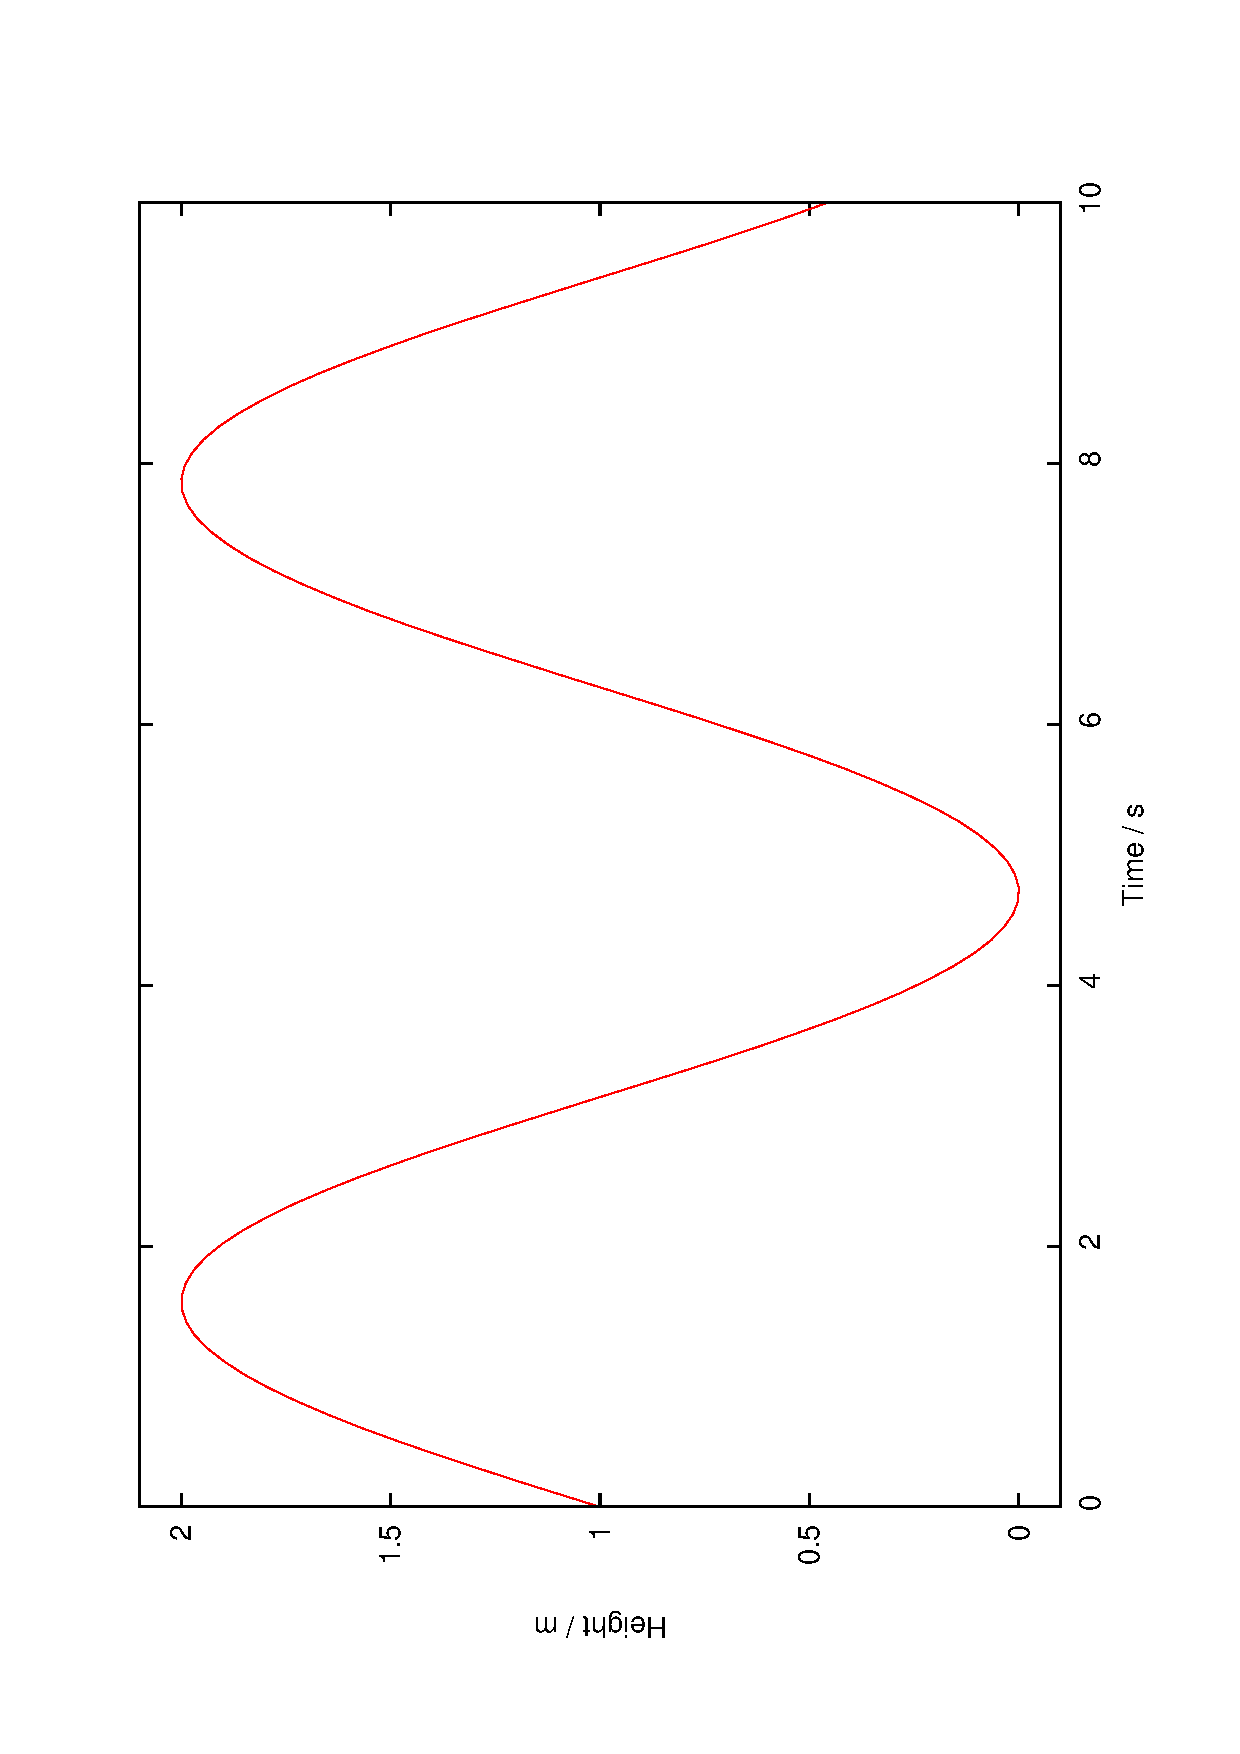
\includegraphics[width=\columnwidth]{example}
%     \caption{This is an example figure. Captions appear below each figure.
% 	Give enough detail for the reader to understand what they're looking at,
% 	but leave detailed discussion to the main body of the text.}
%     \label{fig:example_figure}
% \end{figure}

% % Example table
% \begin{table}
% 	\centering
% 	\caption{This is an example table. Captions appear above each table.
% 	Remember to define the quantities, symbols and units used.}
% 	\label{tab:example_table}
% 	\begin{tabular}{lccr} % four columns, alignment for each
% 		\hline
% 		A & B & C & D\\
% 		\hline
% 		1 & 2 & 3 & 4\\
% 		2 & 4 & 6 & 8\\
% 		3 & 5 & 7 & 9\\
% 		\hline
% 	\end{tabular}
% \end{table}


% \section{Conclusions}

% The last numbered section should briefly summarise what has been done, and describe
% the final conclusions which the authors draw from their work.

% \section*{Acknowledgements}

% The Acknowledgements section is not numbered. Here you can thank helpful
% colleagues, acknowledge funding agencies, telescopes and facilities used etc.
% Try to keep it short.

% %%%%%%%%%%%%%%%%%%%%%%%%%%%%%%%%%%%%%%%%%%%%%%%%%%
% \section*{Data Availability}

 
% The inclusion of a Data Availability Statement is a requirement for articles published in MNRAS. Data Availability Statements provide a standardised format for readers to understand the availability of data underlying the research results described in the article. The statement may refer to original data generated in the course of the study or to third-party data analysed in the article. The statement should describe and provide means of access, where possible, by linking to the data or providing the required accession numbers for the relevant databases or DOIs.


\section{Introduction}
\hspace{\parindent}Neutron stars consist of extremely dense matter, the study of which is important for our understanding of nuclear physics. To investigate the internal structure of these stars we must find ways to probe them using observational phenomena. Short gamma-ray bursts (sGRBs)~\cite{d2015short} are one such phenomena that, while their origins are uncertain, likely originate from the merging of binary neutron stars. These bursts are characterised by a large peak in the gamma-ray count that lasts for $\sim 1$ second or less. Around 10\% of sGRBs are preceded by a 'precursor' flare~\cite{troja2010precursors}. These precursor flares can be identified as a lower, separate peak in the gamma-ray count a short time ($\sim 0.1-1.0$ s) before the main peak~\cite{zhong2019precursors}. In this paper we will investigate the constraints that can be applied to nuclear physics parameters by one possible cause of precursors: resonant shattering flares.

\hspace{\parindent}In the last few years multi-messenger observations of neutron star mergers have provided insight into the origin of sGRBs. In particular, the detection of the gravitational wave signals GW170817~\cite{abbott2017merger} and GW190425~\cite{abbott2020gw190425} (which are thought to originate from mergers) has provided a new angle from which to investigate neutron stars. Here, we use the frequency of gravitational waves to investigate the possibility of a relationship between precursor flares and the modes of oscillation within a neutron star.%second mention of how we use precursors, but have yet to actually explain what we are doing -> but the last sentence of 1st and 2nd paragraph elsewhere (at the end of the introduction?)

\hspace{\parindent}Within a star the bulk motion of matter can be described as a linear combination of an infinite set of oscillation modes~\cite{smeyers2011linear}. Each mode oscillates at a certain frequency, which is value that allows it to obey the boundary conditions for the displacement of matter at both the surface and core of the star. These oscillations can be driven by external gravitational fields, such as that of a binary partner. The frequency and radial profile of the modes are strongly dependant on the internal structure of the star, with different modes being dependant on different properties, such as pressure or shear forces.%mention that excitation can also occur in close encounters in globular clusters?


%define core and crust (and ocean)? or assume reader knows what they are. Might be useful for explaining that the crust has a limit to how much strain it can take.





\subsection{Resonant Shattering Flares}
\hspace{\parindent}During the in-spiral of binary neutron stars the oscillation modes can become excited by the tidal forces from the binary partner. The amount of energy deposited in a specific mode is determined by its overlap with the tidal field, with a stronger overlap giving it more energy. As the stars' orbits get smaller, the frequency of the orbit (and hence the gravitational wave frequency) increases. When the orbital frequency matches a mode's frequency it may become resonantly excited, causing the oscillations to rapidly grow in magnitude~\cite{tsang2012resonant}~\cite{tsang2013shattering}.

\hspace{\parindent}The theory of resonant shattering flares is that if the overlap between the tidal field and an oscillation mode is great enough, the resonant excitation of that mode may cause the neutron star crust to become deformed~\cite{troja2010precursors}. If this deformation becomes large enough the strain in the crust may exceed its limit, causing it to fracture. These fractures deposit seismic energy in the crust which could cause it to shatter, creating high frequency oscillations that couple to the star's magnetic field, causing it to release a precursor flare shortly before the main sGRB.%explain RSF process better?

\hspace{\parindent}Using multi-messenger observations of neutron star mergers, it is possible that the gravitational wave frequencies at which precursor flares occur could be found. In order for a mode to experience resonant excitation, the frequency of the gravitational waves (i.e. the orbital frequency) must be similar to the oscillation frequency of that mode. Therefore, by using a variety of nuclear models to calculate the frequency of a mode that has a strong overlap with the tidal field, the nuclear parameters of those models could be restricted to those that result in a mode frequency which closely matches the observed gravitational wave frequency during the precursor flare. 

\hspace{\parindent}Of particular interest to the RSF process is the interface (i) mode. This mode is caused by the discontinuity between the crust and core and has a strong overlap with the tidal field~\cite{tsang2012resonant}. This makes it a good candidate for the source of RSFs as less time will be needed at resonance for it to reach the elastic limit for the crust to begin to fracture. In this work we will focus on finding the relationship between the frequency of the i-mode and the nuclear symmetry energy parameters.








\subsection{Nuclear Symmetry Energy and Neutron Star Structure}
\hspace{\parindent}The mode frequencies are dependant on the neutron star equation of state (EoS), the relationship between the energy density and pressure inside the star. At low densities the EoS can be accurately calculated by using the properties of experimentally measured nuclei~\cite{baym1971ground}. However, at the extreme densities found in neutron stars we must rely on nuclear models to calculate the EoS, with different models giving significantly different EoSs. In order to reproduce physical results, these models are parameterised with various nuclear properties, such as the symmetry energy parameters. The nuclear symmetry energy is the energy required to convert a proton into a neutron (or vice-versa) when the neutron and proton numbers are equal. At nuclear saturation density (the density of nucleons in a nucleus) the first three symmetry energy parameters are: the symmetry energy
\begin{align}
J=E_{\rm sym}(n_0),    
\label{eq:sym_J}
\end{align}
\noindent its first derivative 
\begin{align}
L=3n_0\frac{\partial E_{\rm sym}(n_b)}{\partial n_b}\biggr\rvert_{n_b=n_0},  
\label{eq:sym_L}
\end{align}
\noindent and its second derivative
\begin{align}
K_{\rm sym}=9n_0^2\frac{\partial^2 E_{\rm sym}(n_b)}{\partial n_b^2}\biggr\rvert_{n_b=n_0},
\label{eq:sym_K}
\end{align}
\noindent where $n_0\approx 0.16$ fm$^{-3}$ is the nuclear saturation density and $n_b$ is the baryon density.

\hspace{\parindent}To investigate the nuclear symmetry energy parameters we generated a set of EoSs spanning a reasonable range of values for $J$ ,$L$ and $K_{\rm sym}$. By calculating the mode frequencies for these EoSs we are able to find the relationship between the symmetry energy parameters and the gravitational wave frequency at which an RSF occurs.







\section{Parameterised Neutron Star Equation of State and Composition}














...

% \begin{figure}
% \centering
% 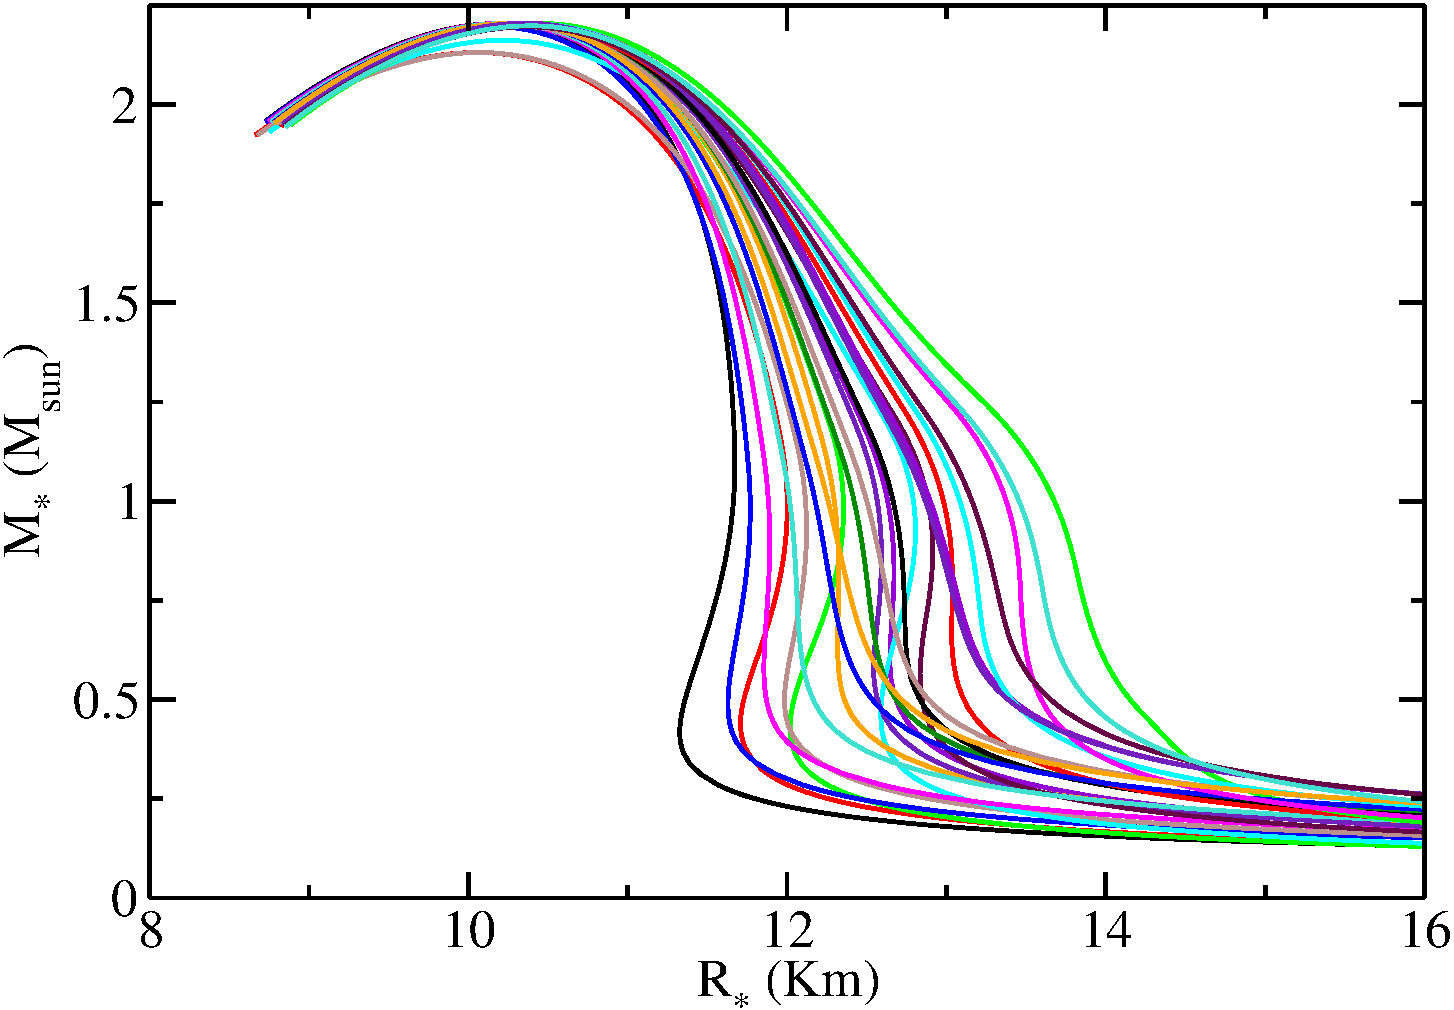
\includegraphics[width=0.45\textwidth,angle=0]{TOVs.pdf}
% \caption{The mass-radius relationships calculated using the TOV equations for all of the $J$, $L$, $K_{\rm sym}$ values.}
% \label{fig:TOVs}
% \end{figure}








\section{Calculation of the Normal Modes}
\hspace{\parindent}Each oscillation mode gives a different profile for the radial and transverse displacements. To calculate this, as well as the mode frequencies, we perturb the equations defining the equilibrium state of neutron star matter. The neutron stars involved in mergers are old and therefore will have cooled and spun down, so we assume the temperature is low throughout the star and ignore effects of rotation. We also assume that the periods of the modes that we are interested in are significantly lower that the beta equilibrium timescale. Unless otherwise stated, we have use $1.4M_{\odot}$ neutron stars. Finally, we ignore terms that are non-linear in perturbations because they are small and therefore non-linear terms are negligible.
% low temperature or zero temperature? is 'spun down' correct?



%explain Eulerian vs Lagrangian perturbations?
\subsection{Linear Perturbation Equations}
\hspace{\parindent}Following the methodology of~\cite{mcdermott1988nonradial}, the equations governing the displacement caused by the modes of oscillation can be derived from the equations for mass continuity, momentum conservation, and Poisson's equation:
\begin{align}
\frac{\partial\rho}{\partial t}+\nabla\cdot(\rho v)=0,
\label{eq:continuity_eqn}
\end{align}
\begin{align}
\frac{\partial v}{\partial t}=(v\cdot \nabla)v=\frac{1}{\rho}\nabla\cdot\sigma-\nabla\Phi,
\label{eq:momentum_eqn}
\end{align}
\begin{align}
\nabla^2\Phi=4\pi G\rho,
\label{eq:Poisson_eqn}
\end{align}
\noindent where $\rho$ is the energy density, $v$ is the velocity of the matter, $\sigma$ is the stress tensor, and $\Phi$ is the gravitational potential. By adding a small perturbation to each of the quantities in these equations (eg: $\rho\rightarrow\rho+\delta\rho$), and ignoring terms that are non-linear in perturbations, these three equations can be used to obtain the wave equation
\begin{align}\nonumber
&&\omega^2u=-\nabla\left(\frac{\Gamma_1 p}{\rho}\nabla\cdot u\right)-\nabla\left(\frac{1}{\rho}u\cdot\nabla p\right)-\hat{r}A\frac{\Gamma_1 p}{\rho}\nabla\cdot u\\\nonumber
&&+\frac{1}{\rho}\biggr(\nabla\left(\frac{2}{3}\mu\nabla\cdot u\right)-\left(\nabla\mu\cdot\nabla\right)u-\nabla\left(u\cdot\nabla\mu\right)\\
&&+\left(u\cdot\nabla\right)\nabla\mu-\mu\left(\nabla^2 u+\nabla\left(\nabla\cdot u\right)\right)\biggr),
\label{eq:wave_eqn}
\end{align}
where $u(x,t)$ is the Lagrangian displacement (the displacement of the mass element initially located at $x$),
\begin{align}
A=\frac{1}{\rho}\frac{d\rho}{dr}-\frac{1}{\Gamma_1P}\frac{dP}{dr}
\label{eq:schwartz_descrim}
\end{align}
\noindent is the Schwarzschild discriminant, and
\begin{align}
\Gamma_1=\left(\frac{\partial\:ln(P)}{\partial\:ln(\rho)}\right)_s
\label{eq:adiabatic_index}
\end{align}
\noindent is the adiabatic index when the composition of the star is frozen. The non-diagonal terms of the stress tensor have become the shear modulus, which we calculated using~\cite{strohmayer1991shear}
\begin{align}
\mu=\frac{0.1194}{1+17810\left(\frac{ak_bT}{\left(Ze\right)^2}\right)^2}\frac{n_i\left(Ze\right)^2}{a},
\label{eq:mu_1991}
\end{align}
\noindent where $T$ is the temperature, $n_i$ is the ion density, $Z$ is the proton number of the nuclei, and 
\begin{align}
a=\left(\frac{3}{4\pi n_i}\right)^{\frac{1}{3}}.
\label{eq:mu_1991_a}
\end{align}
\noindent We have also taken the Cowling approximation~\cite{cowling1941non}. This approximation states that, since the mass of a star is concentrated in its centre, the displacement of matter that is not close to the centre does not significantly alter the gravitational potential and therefore $\Phi '\approx 0$. The time dependence of the perturbed quantities was assumed to be of the form $e^{i\omega t}$, with $\omega$ being the oscillation frequency of the mode. This can be used to separate the time and position dependencies of the Lagrangian displacement to get
\begin{align}
u(x,t)=\xi(x)e^{i\omega t}.
\label{eq:time_seperation}
\end{align}
\noindent In spherical coordinates this can be further separated into radial and transverse components:
\begin{align}
\xi_r=U(r)Y_{lm},\;\;\;\xi_{\theta}=V(r)\frac{\partial Y_{lm}}{\partial\theta},\;\;\;\xi_{\phi}=\frac{V(r)}{sin(\theta)}\frac{\partial Y_{lm}}{\partial\phi},
\label{eq:xi_seperation}
\end{align}
\noindent with $U(r)$ being the radial displacement, $V(r)$ being the transverse displacement, and $Y_{lm}$ being the spherical harmonics.

\hspace{\parindent}By using the separation of variables given in equations \ref{eq:time_seperation} and \ref{eq:xi_seperation}, equation \ref{eq:wave_eqn} becomes a set of 4 equations:% (or 5 without the Cowling approximation) 
\begin{align}\nonumber
&&\rho\omega^2U=\rho\frac{d\hat{\chi}}{dr}-A\Gamma_1 p\hat{\alpha}-\frac{d}{dr}\left(\frac{1}{3}\mu\hat{\alpha}\right)+\frac{d\mu}{dr}\left(\hat{\alpha}-2\frac{dU}{dr}\right)\\
&&-\mu\left(\frac{1}{r^2}\frac{d}{dr}\left( r^2\frac{dU}{dr}\right)-\frac{l(l+1)}{r^2}U+\frac{2l(l+1)}{r^2}V\right),
\label{eq:Ueqn}
\end{align}
\begin{align}\nonumber
&&\rho\omega^2V=\rho\frac{\hat{\chi}}{r}-\frac{1}{3}\frac{\mu\hat{\alpha}}{r}-\frac{d\mu}{dr}\left(\frac{dV}{dr}-\frac{V}{r}+\frac{U}{r}\right)\\
&&-\mu\left(\frac{1}{r^2}\frac{d}{dr}\left(r^2\frac{dV}{dr}\right)-\frac{l(l+1)}{r^2}V+\frac{2}{r^2}U\right),
\label{eq:Veqn}
\end{align}
% \begin{align}
% \frac{1}{r^2}\frac{d}{dr}\left(r^2\frac{d\hat{\Phi}'}{dr}\right)-\frac{l(l+1)}{r^2}\hat{\Phi}'=4\pi G\left(U\frac{d\rho}{dr}+\hat{\alpha}\rho\right),
% \label{eq:Phihat_eqn}
% \end{align}
\noindent where:
\begin{align}
\hat{\alpha}=\frac{1}{r^2}\frac{d}{dr}(r^2U)-\frac{l(l+1)}{r}V,
\label{eq:alphahat}
\end{align}
\begin{align}
\hat{\chi}=-\frac{\Gamma_1p}{\rho}\hat{\alpha}-\frac{1}{\rho}\frac{\partial p}{\partial r}U.
\label{eq:chihat}
\end{align}



\hspace{\parindent}For the fluid core of a neutron star, equations \ref{eq:Ueqn}-\ref{eq:chihat} are further simplified because in a fluid the shear modulus must be zero. By using $\mu=0$, and be rewriting $U$ and $V$ as the dimensionless variables
\begin{align}
y_1=\frac{U}{r},\;\;\;\;y_2=\frac{\omega^2V}{g}
\label{eq:y1y2}
\end{align}
\noindent (where $g=\frac{1}{\rho}\frac{dP}{dr}$), equations \ref{eq:Ueqn}-\ref{eq:chihat} can be rewritten as a pair of coupled differential equations:
\begin{align}
\left(1+\tilde{V}\right)\frac{dy_1}{dx}=\left(\frac{\tilde{V}}{\Gamma_1}-3\right)y_1+\left(\frac{l(l+1)}{c_1\Omega^2}-\frac{\tilde{V}}{\Gamma_1}\right)y_2,
\label{eq:McDy1}
\end{align}
\begin{align}
\left(1+\tilde{V}\right)\frac{dy_2}{dx}=\left(c_1\Omega^2+Ar\right)y_1+\left(1-\tilde{U}-Ar\right)y_2,
\label{eq:McDy2}
\end{align}
\noindent where the equilibrium properties of the star are: 
\begin{align}\nonumber
\tilde{U}=\frac{d\:ln\left(M_r\right)}{d\:ln\left(r\right)}=4\pi r^2\rho\frac{r}{M_r},\;\;\;c_1=\left(\frac{r}{R_*}\right)^3\frac{M_*}{M_r},\;\;\;\Omega^2=\frac{\omega^2R_*^3}{GM_*},
% \label{eq:eqbm_properties1}
\end{align}
\begin{align}\nonumber
\tilde{V}=-\frac{d\:ln\left(P\right)}{d\:ln\left(r\right)}=-\frac{G\rho M_r}{rP}\left(1+\frac{P}{\rho c^2}\right)\left(1+\frac{4\pi r^3 P}{M_r c^2}\right)\left(1-\frac{2GM_r}{rc^2}\right)^{-1},
% \label{eq:eqbm_properties2}
\end{align}




\hspace{\parindent}For the solid crust the shear modulus is not zero, and therefore we obtain a set of four coupled differential equations:
\begin{align}
\left(1+\tilde{V}\right)\frac{dz_1}{dx}=-\left(1+2\frac{\alpha_2}{\alpha_3}\right)z_1+\frac{1}{\alpha_3}z_2+l\left(l+1\right)\frac{\alpha_2}{\alpha_3}z_3,
\label{eq:z1dr}
\end{align}
\begin{align}\nonumber
&&\left(1+\tilde{V}\right)\frac{dz_2}{dx}=\left(-\tilde{V}c_1\Omega^2-4\tilde{V}+\tilde{U}\tilde{V}+12\Gamma_1\frac{\alpha_1}{\alpha_3}\right)z_1\\\nonumber
&&+\left(\tilde{V}-4\frac{\alpha_1}{\alpha_3}\right)z_2+l\left(l+1\right)\left(\tilde{V}-6\Gamma_1\frac{\alpha_1}{\alpha_3}\right)z_3\\
&&+l\left(l+1\right)z_4,
\label{eq:z2dr}
\end{align}
\begin{align}
\left(1+\tilde{V}\right)\frac{dz_3}{dx}=-z_1+\frac{1}{\alpha_1}z_4,
\label{eq:z3dr}
\end{align}
\begin{align}\nonumber
&&\left(1+\tilde{V}\right)\frac{dz_4}{dx}= \biggr(-\tilde{V}c_1\Omega^2+\frac{2}{\alpha_3}\biggr((2l(l+1)-1)\alpha_1\alpha_2\\\nonumber
&&+2(l(l+1)-1)\alpha_1^2\biggr)\biggr)z_3\\
&&+\left(\tilde{V}-6\Gamma_1\frac{\alpha_1}{\alpha_3}\right)z_1-\frac{\alpha_2}{\alpha_3}z_2+(\tilde{V}-3)z_4,
\label{eq:z4dr}
\end{align}
\noindent where $\alpha_1=\frac{\mu}{\rho}$, $\alpha_2=\Gamma_1-\frac{2}{3}\frac{\mu}{\rho}$, $\alpha_3=\Gamma_1+\frac{4}{3}\frac{\mu}{\rho}$, and the dimensionless variables are 
\begin{align}
&z_1=\frac{U}{r},&z_2=\frac{1}{\rho}\left((\Gamma_1p-\frac{2}{3}\mu)\hat{\alpha}+2\mu\frac{dU}{dr}\right),\\
&z_3=\frac{V}{r},&z_4=\frac{\mu}{p}\left(\frac{dV}{dr}-\frac{V}{r}+\frac{U}{r}\right).
\label{eq:z1z2z3z4}
\end{align}
\noindent $z_1$ is the radial displacement, $z_2$ is proportional to the radial traction, $z_3$ is the transverse displacement, and $z_4$ is proportional to the transverse traction.



\hspace{\parindent}At the boundary between the solid crust and the fluid core (and the boundary between the fluid surface ocean and the solid crust), there are three jump conditions that must be satisfied:
\begin{align}
z_1=y_1,
\label{eq:jump1}
\end{align}
\begin{align}
z_2=\tilde{V}(y_1-y_2),
\label{eq:jump2}
\end{align}
\begin{align}
z_4=0.
\label{eq:jump3}
\end{align}
\noindent The first two of these conditions can be combined to obtain $\frac{z_2}{z_1}=\tilde{V}\left(1-\frac{y_2}{y_1}\right)$, resulting in two conditions and two eigenvalues, $\Omega$ and $z_3$ at the top of the crust.  %'z_3 at the top of the crust' or 'z_3(R_*)'?



\hspace{\parindent}For any mode the boundary conditions at the centre and surface of the star must be obeyed. The condition at the centre follows from the requirement that $y_1$ and $y_2$ be regular at $r=0$:
\begin{align}
\frac{c_1\Omega^2}{l}y_1-y_2=0.
\label{eq:core_condition}
\end{align}
\noindent The condition at the surface is based on the requirement that the Lagrangian pressure perturbation goes to zero at $r=R_*$:
\begin{align}
\left(\tilde{V}-c_1\Omega^2-4+\tilde{U}\right)y_1+\left(\frac{l(l+1)}{c_1\Omega^2}-\tilde{V}\right)y_2=0,
\label{eq:surface_condition}
\end{align}
\noindent However, this boundary condition is for the surface ocean we skip due to it having a negligible impact on the i-mode. Therefore the surface boundary condition must be combined with the jump conditions (equations \ref{eq:jump1}-\ref{eq:jump3}) to rewrite it as
\begin{align}
z_2=\tilde{V}\left(\frac{\tilde{V}-c_1\Omega^2-4+\tilde{U}}{\frac{l(l+1)}{c_1\Omega^2}-\tilde{V}}+1\right)z_1,
\label{eq:surface_boundary_modified_1}
\end{align}
\begin{align}
z_4=0.
\label{eq:surface_boundary_modified_2}
\end{align}



\hspace{\parindent}We solve for the eigenvalues by choosing initial guesses for them and then using the shooting method to go from the core and surface boundary conditions to the crust-core transition. We then adjust the eigenvalues until the jump conditions are satisfied, indicating that a mode has been found. Figure \ref{fig:trace_minima} shows the eigenvalues at which each of the jump conditions are satisfied, with modes being located at the places where they coincide.

\begin{figure}
\centering
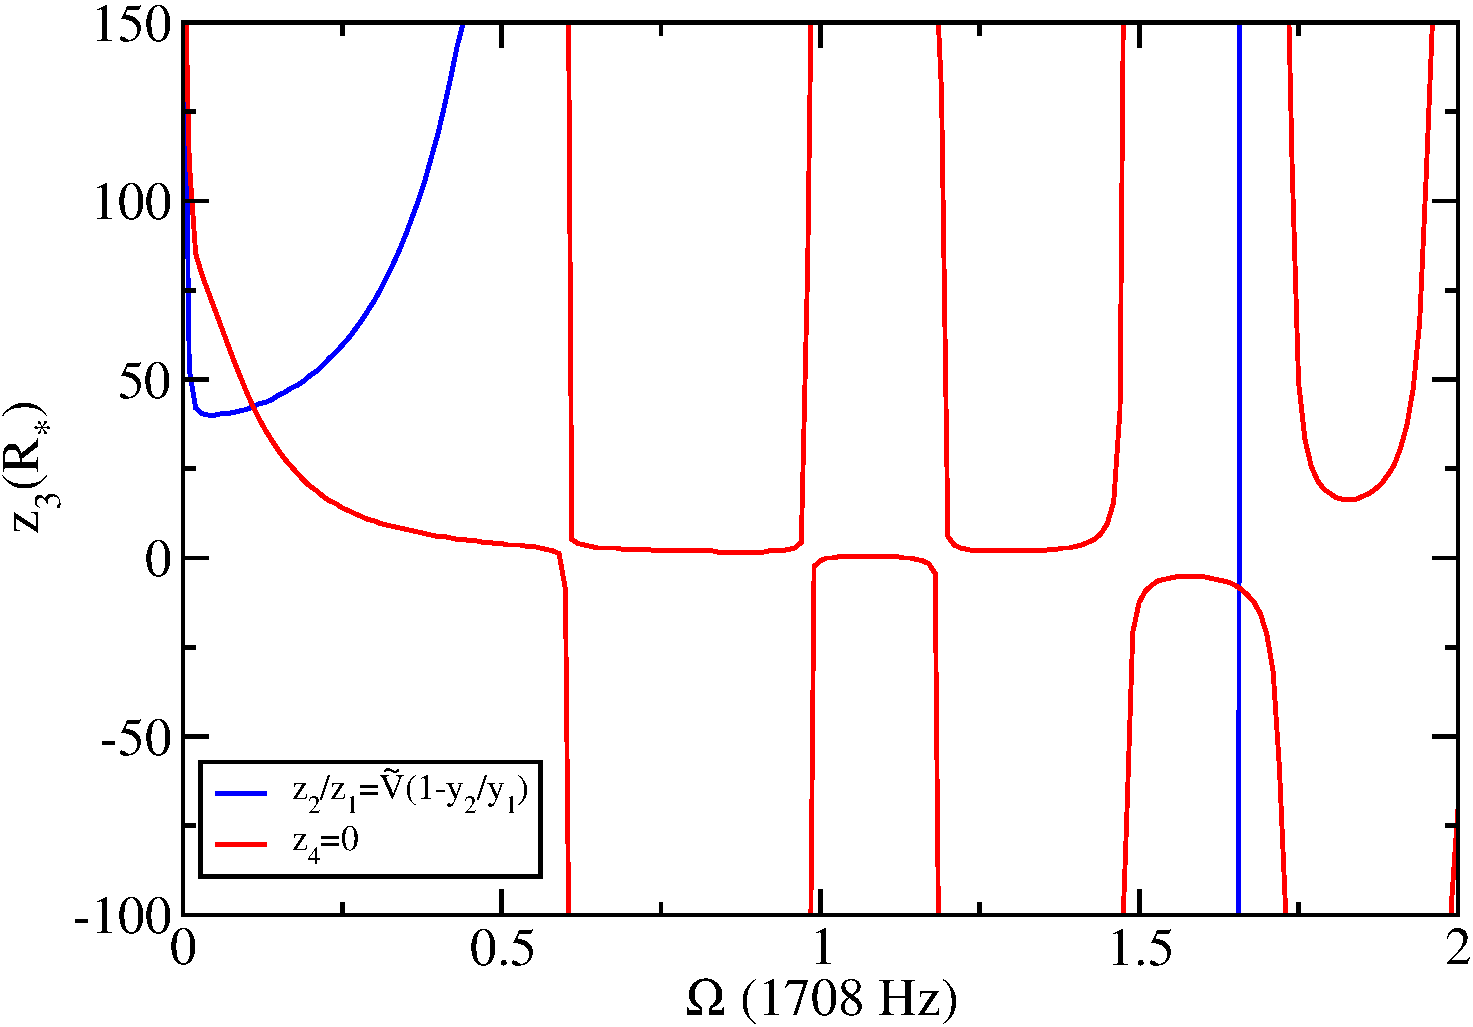
\includegraphics[width=0.45\textwidth,angle=0]{minima_new}
\caption{The zeros of the error in the jump conditions at the crust-core boundary, showing the location of two modes for the sly4 EoS (the interface and fundamental modes).}
\label{fig:trace_minima}
\end{figure}







\subsection{The Crust-Core Interface Mode}
\hspace{\parindent}The interface mode shown in figure \ref{fig:imode_sly4} has its radial displacement peaking at the crust-core boundary, which is what we would expect because the i-mode is caused by the discontinuity between the crust and core. For the sly4 EoS, its eigenvalues are $\Omega=0.1104$ and $z_3(R_*)=42.39$ (as can be seen in figure \ref{fig:trace_minima}), giving the mode a frequency of $188.5$ Hz. The transverse displacement in the core is small, while in the crust it discontinuously jumps to become large. This makes the i-mode a good candidate for an RSF because more of its energy will go into deforming the crust.

\begin{figure}
\centering
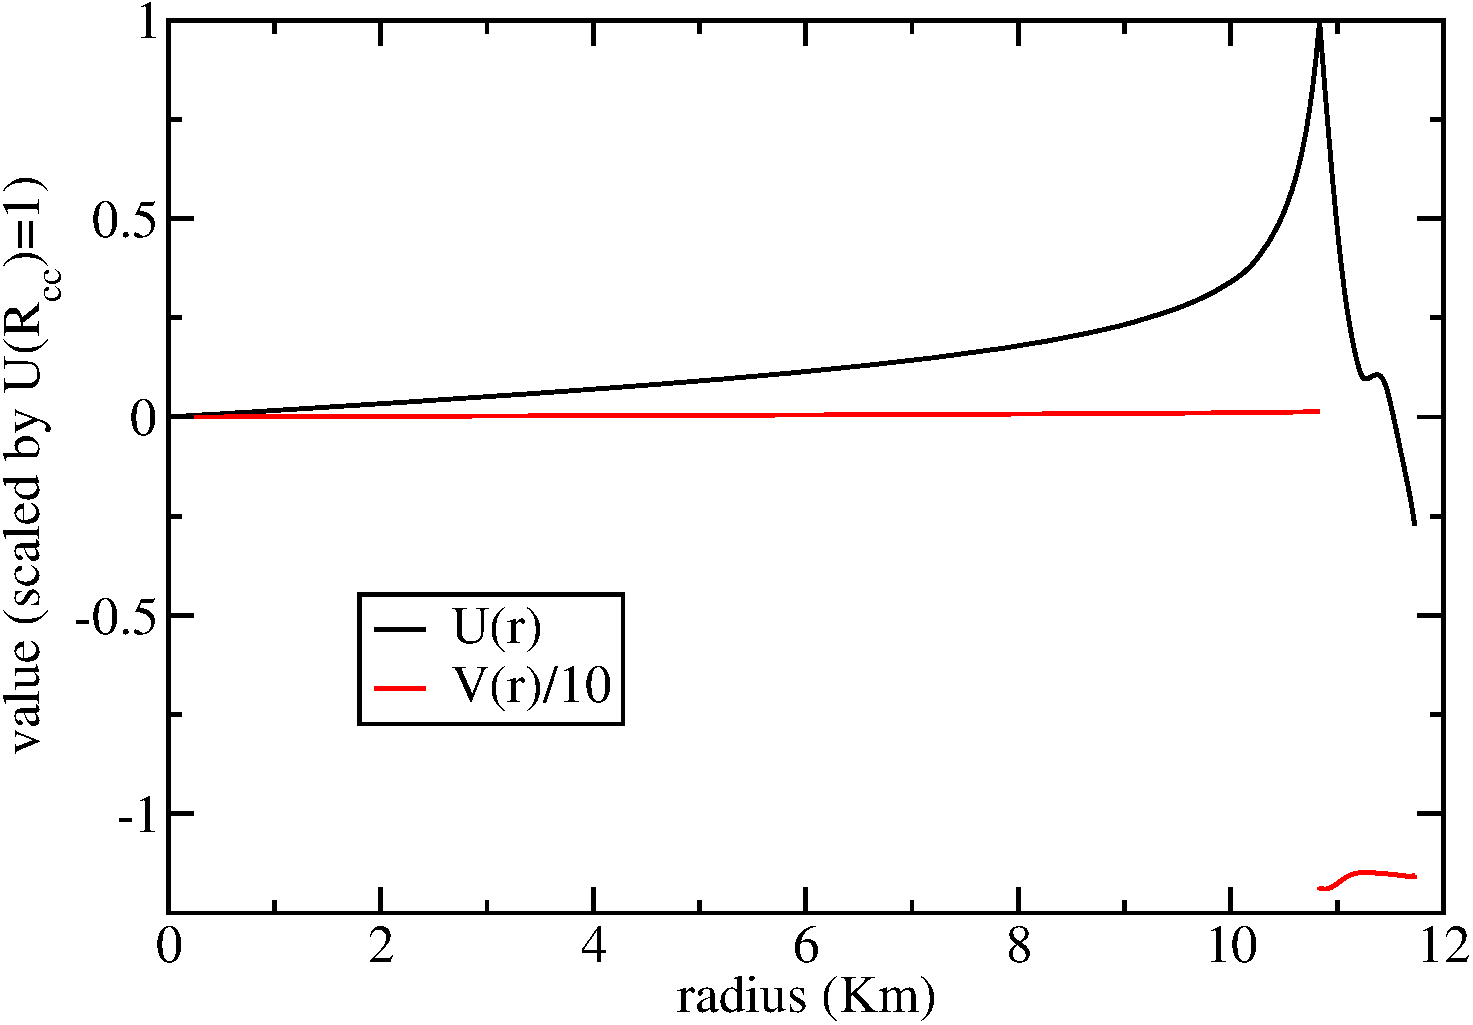
\includegraphics[width=0.45\textwidth,angle=0]{sly4_imode}
\caption{The 2i mode for the sly4 equation of state. $V(r)$ has been reduced by an order of magnitude so that it can be plotted alongside $U(r)$.}
\label{fig:imode_sly4}
\end{figure}

\hspace{\parindent}The i-mode has a strong dependence on the shear modulus in the crust, and more specifically at the crust-core transition. We investigated this dependence by considering a shear modulus scaled by 
\begin{align}
\tilde{\mu} = B \mu,
\end{align}
\noindent where the constant $B$ was varied to determine its impact on the i-mode. Figure \ref{fig:mu_B} shows the relationship between $B$ and the i-mode frequency. The constant which controls the scaling due to temperature was not varied because for most of the crust $1>>17810\left(\frac{ak_bT}{\left(Ze\right)^2}\right)^2$, meaning that the temperature's impact on the shear modulus is small. Therefore this constant would need to be very large to have a noticeable impact on it. Modifying the shear modulus by varying $B$ is very artificial because it is strongly linked to the equilibrium properties of the star, and so the other properties would also have to be changed for this to be realistic. Therefore, only changing the shear modulus should only be seen as a rough guide to its impact on the frequency.

\begin{figure}
\centering
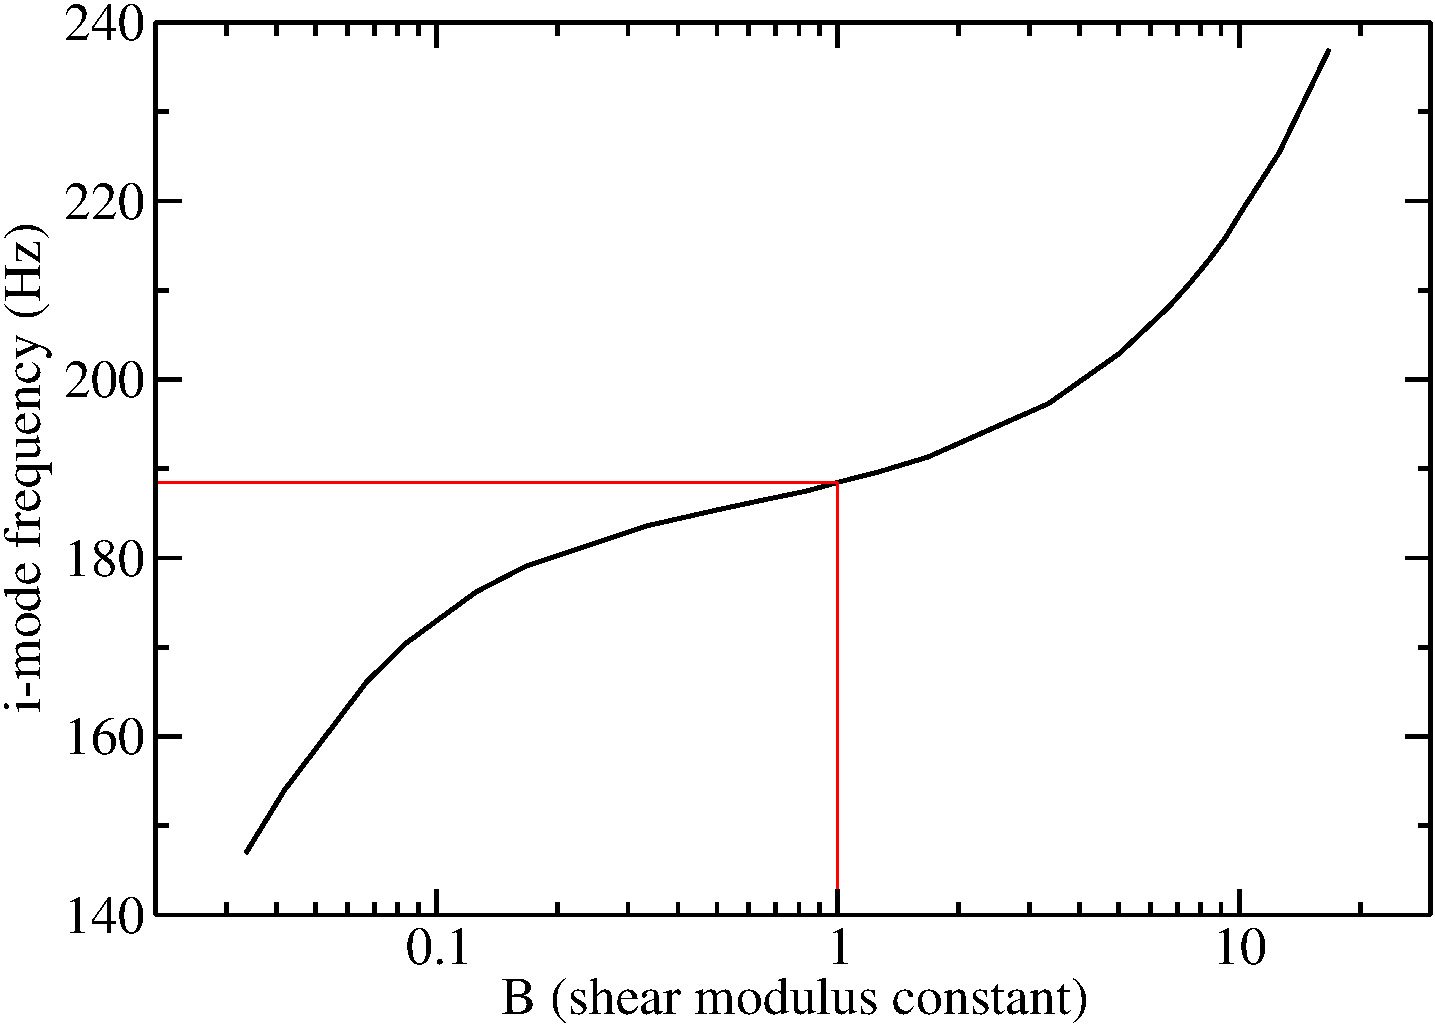
\includegraphics[width=0.45\textwidth,angle=0]{shear_mod_vs_freq_2}
\caption{The change in i-mode frequency caused by scaling the shear modulus with a constant. The red lines indicate the result for $B=1$ (which gives equation \ref{eq:mu_1991}).}
\label{fig:mu_B}
\end{figure}










\section{Results}
\hspace{\parindent}Figure \ref{fig:f_vs_Rcc_R*} shows the relationship between the frequency of the i-mode and both the location of the crust-core transition and the total radius of the star for the sly4 EoS. This figure was created by varying the central pressure of the neutron star and using the TOV equations to find $R_*$ and $R_{cc}$. Then the i-mode frequency was calculated each of the central pressures. The crust-core transition density was also varied, since this also effects the shear modulus at the transition. Three different values were manually inputted to investigate its effect on the i-mode frequency, and from the figure it can been seen that the relationship between the star's radius, $n_{b,cc}$ and the frequency is not simple, particularly for higher $n_{b,cc}$ values. For $n_{b,cc}=6.5\times10^{37}$ cm$^{-3}$ there is a maximum i-mode frequency of $239$ Hz at around $R_*=12.5$ Km, which places an upper limit on the frequency. However, the mass of a neutron star with this radius is very low ($0.45$ M$_{\odot}$), and therefore the i-mode frequency would likely be significantly lower than this value. If this maximum appears for the EoSs parameteried by $J$, $L$ and $K_{\rm sym}$, we could use it to constrain $J$, $L$ and $K_{\rm sym}$ for stars whose mass is not known.
%check this last sentence, what can we learn from this figure?

\begin{figure}
\centering
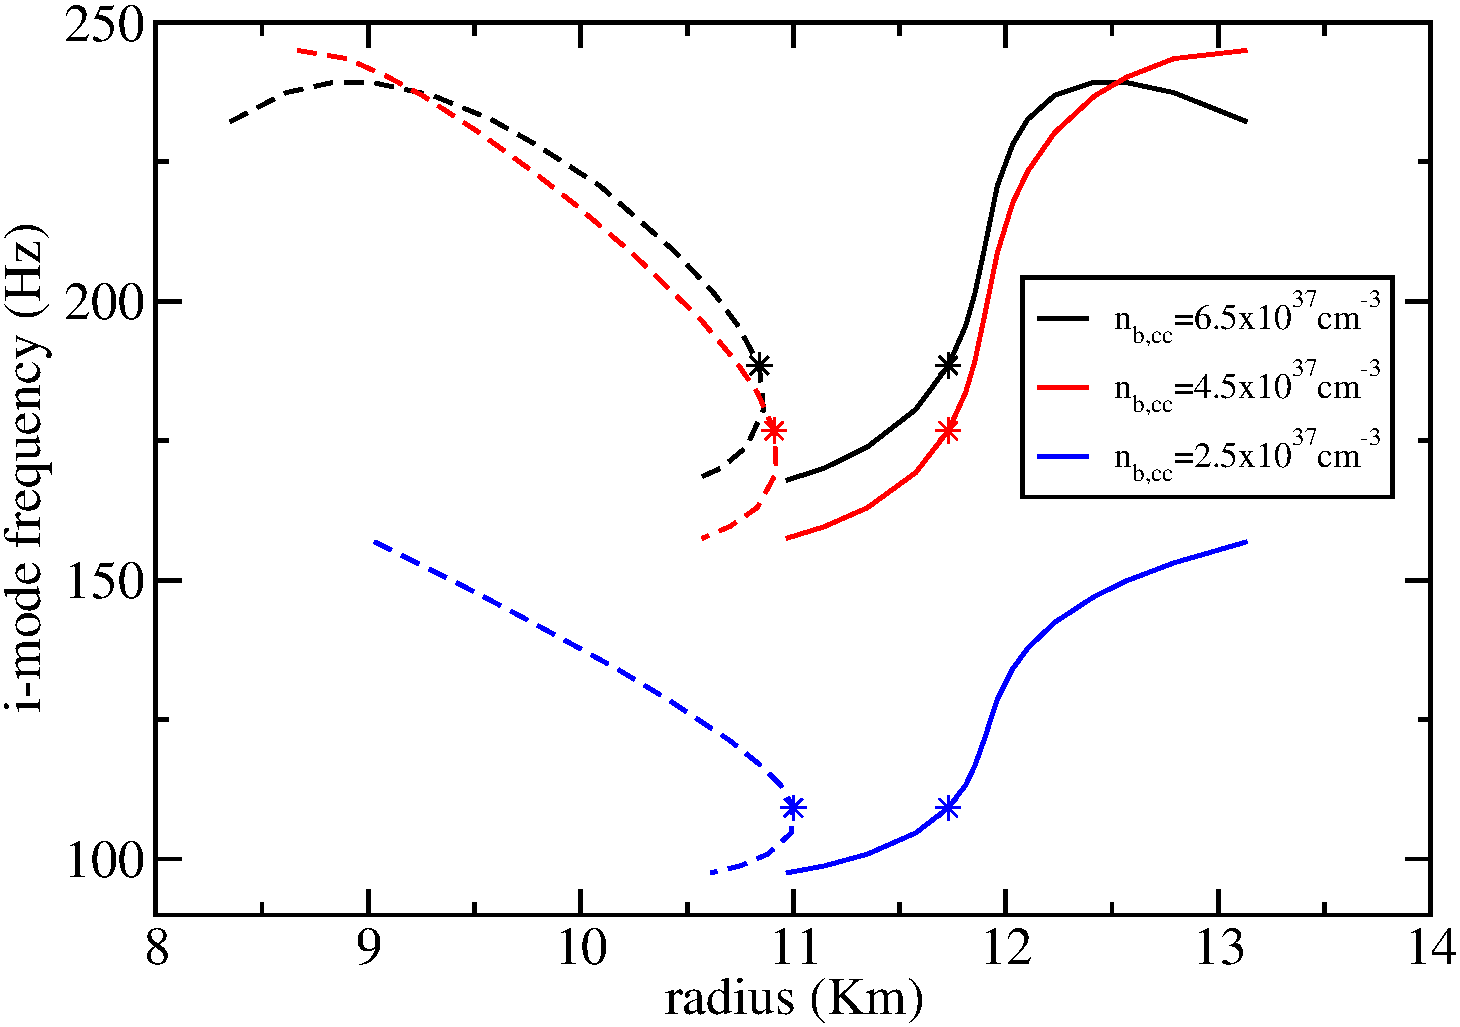
\includegraphics[width=0.45\textwidth,angle=0]{f_Rstar_Rcc_2}
\caption{The frequency of the i-mode for varying neutron star mass and radius. The figure shows both the total radius (solid lines) and crust-core radius (dashed lines) for each frequency. The stars indicate $1.4$ solar masses neutron stars. Increasing total radius causes the central pressure and total mass to decrease.}%check this, 'for each frequency' doesn't sound right...
\label{fig:f_vs_Rcc_R*}
\end{figure}




\subsection{Interface Mode dependence on Nuclear Parameters}
\hspace{\parindent}We calculated the i-mode frequency for our set of EoSs parameterised by $J$, $L$ and $K_{\rm sym}$, and then interpolated between them to obtain frequency contours in the $J,L$ plane. This is shows in figure \ref{fig:freq_contours}, with the two graphs showing either end of a reasonable $K_{\rm sym}$ range. From this we see that changes in $L$ and $K_{\rm sym}$ have larger impacts on the the i-mode frequency than changes in $J$ do. This is what we would expect because the matter in neutron stars is highly asymmetric.



\begin{figure}
\centering
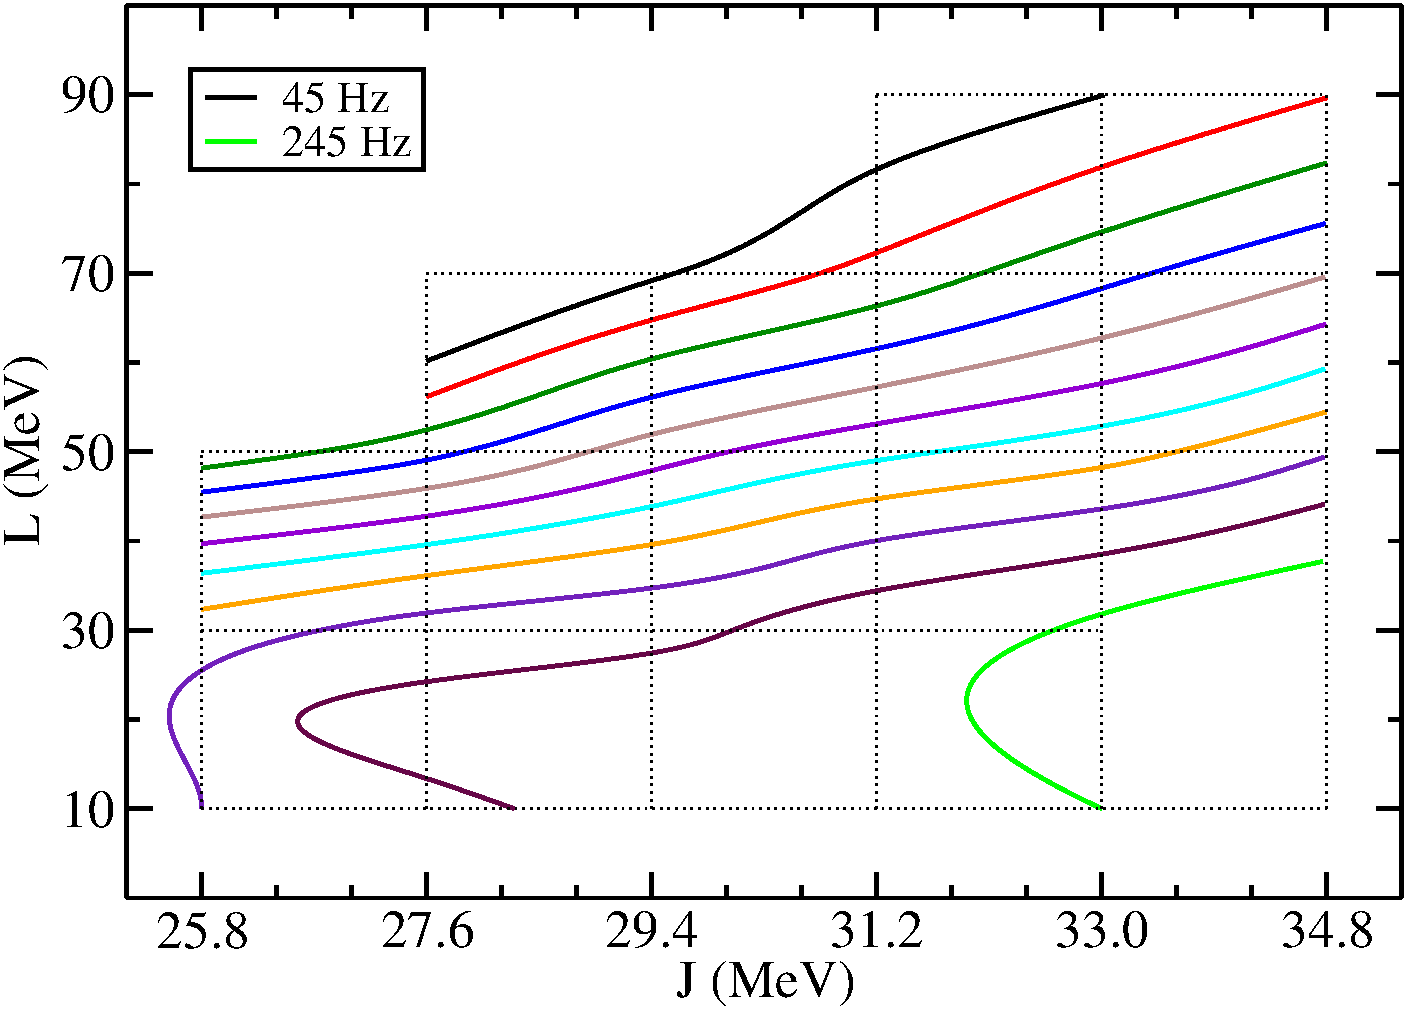
\includegraphics[width=0.45\textwidth,angle=0]{contours_20gap_K40}
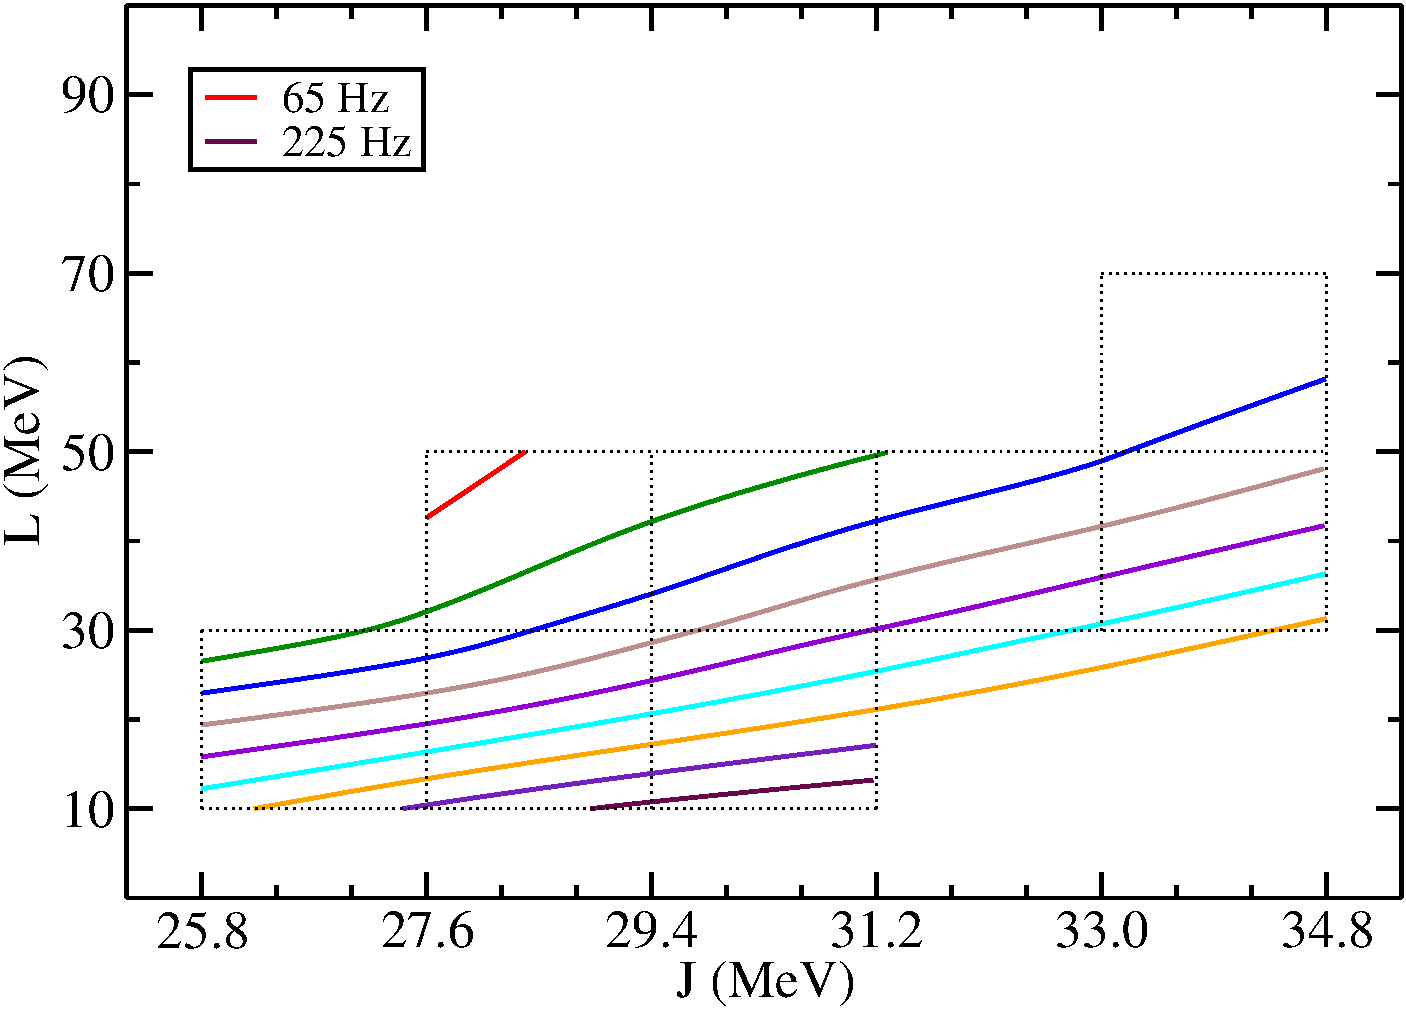
\includegraphics[width=0.45\textwidth,angle=0]{contours_20gap_Km200}
\caption{Frequency contours in the $J,L$ plane, with the first figure being for $K_{\rm sym}=40$ MeV, and the second for $K_{\rm sym}=-200$ MeV. The gaps between the contours are $20$ Hz. The grid points indicate the results of the EoSs, between which the frequency was interpolated.}
\label{fig:freq_contours}
\end{figure}








\subsection{Constraining $J$, $L$, and $K_{\rm sym}$ with an RSF detection}
\hspace{\parindent}The timescale over which resonant excitation of a mode can occur is calculated as \cite{tsang2012resonant}
\begin{align}
t_{\rm res}\sim 8\times10^{-2}\text{s}\left(\frac{\mathcal{M}}{1.2\text{M}_{\odot}}\right)^{\frac{-5}{6}}\left(\frac{f_{\rm mode}}{100 \text{ Hz}}\right)^{\frac{-11}{6}},
\label{res_timescale}    
\end{align}
\noindent where $\mathcal{M}=\frac{M_1^{\frac{3}{5}}M_2^{\frac{3}{5}}}{(M_1+M_2)^{\frac{1}{5}}}$ is the chirp mass. This can be combined with the rate of change of the gravitational wave frequency
\begin{align}
\Dot{f}_{\rm gw}=\frac{f_{\rm gw}}{4.7\times10^{-3}\text{s}}\left(\frac{\mathcal{M}}{1.2\text{M}_{\odot}}\right)^{\frac{5}{3}}\left(\frac{f_{\rm gw}}{1000 \text{ Hz}}\right)^{\frac{8}{3}},
\label{res_timescale}    
\end{align}
\noindent where $f_{\rm gw}\approx f_{\rm mode}$. This gives a simple estimate of the range of frequencies over which resonance can occur:
\begin{align}
\delta f\sim t_{\rm res}\Dot{f}_{\rm gw}\sim3.7\text{Hz}\left(\frac{\mathcal{M}}{1.2\text{M}_{\odot}}\right)^{\frac{5}{6}}\left(\frac{f_{\rm mode}}{100 \text{ Hz}}\right)^{\frac{11}{6}}.
\label{res_timescale}    
\end{align}
\noindent From this we see that the resonance window gets larger as the frequency increases, with $\delta f$ scaling as $f_{\rm mode}^{\frac{11}{6}}$. For a resonance at $100$ Hz and a chirp mass of $1.2M_{\odot}$ we get a frequency range of $\delta f\sim 3.7$ Hz, while for $150$ Hz we get a range of $\delta f\sim 7.8$ Hz. This means that the spread of the frequency contour in the $J,L$ plane (which is shown in figure \ref{fig:t_res_spread}) is small ($\delta L\approx 0.5-2.0$ MeV). Therefore the main uncertainty will come from the value of $K_{\rm sym}$, which causes a spread of up to $\sim 20$ MeV in $L$ at any given $J$ value (as can be seen in \ref{fig:freq_contours}).
%From this we see that the resonance window gets smaller as the frequency increases, giving a smaller range over which the resonance will be spread. For a resonance at $100$ Hz and a chirp mass of $1M_{\odot}$, $t_{\rm res}\sim 0.093$ s which gives a frequency range of $\delta f\sim 3.15$ Hz. This means that the spread of the contour in the $J,L$, which is shown in figure \ref{fig:t_res_spread} is small, and so the main uncertainty will come from the value of $K_{\rm sym}$, which causes a spread of up to $\sim 20$ MeV in $L$ at any given $J$ value.
%I've used t_res*df/dt to get $\delta$ f, which would give $\delta$ f proportional to f^(11/6). Is this correct?

\begin{figure}
\centering
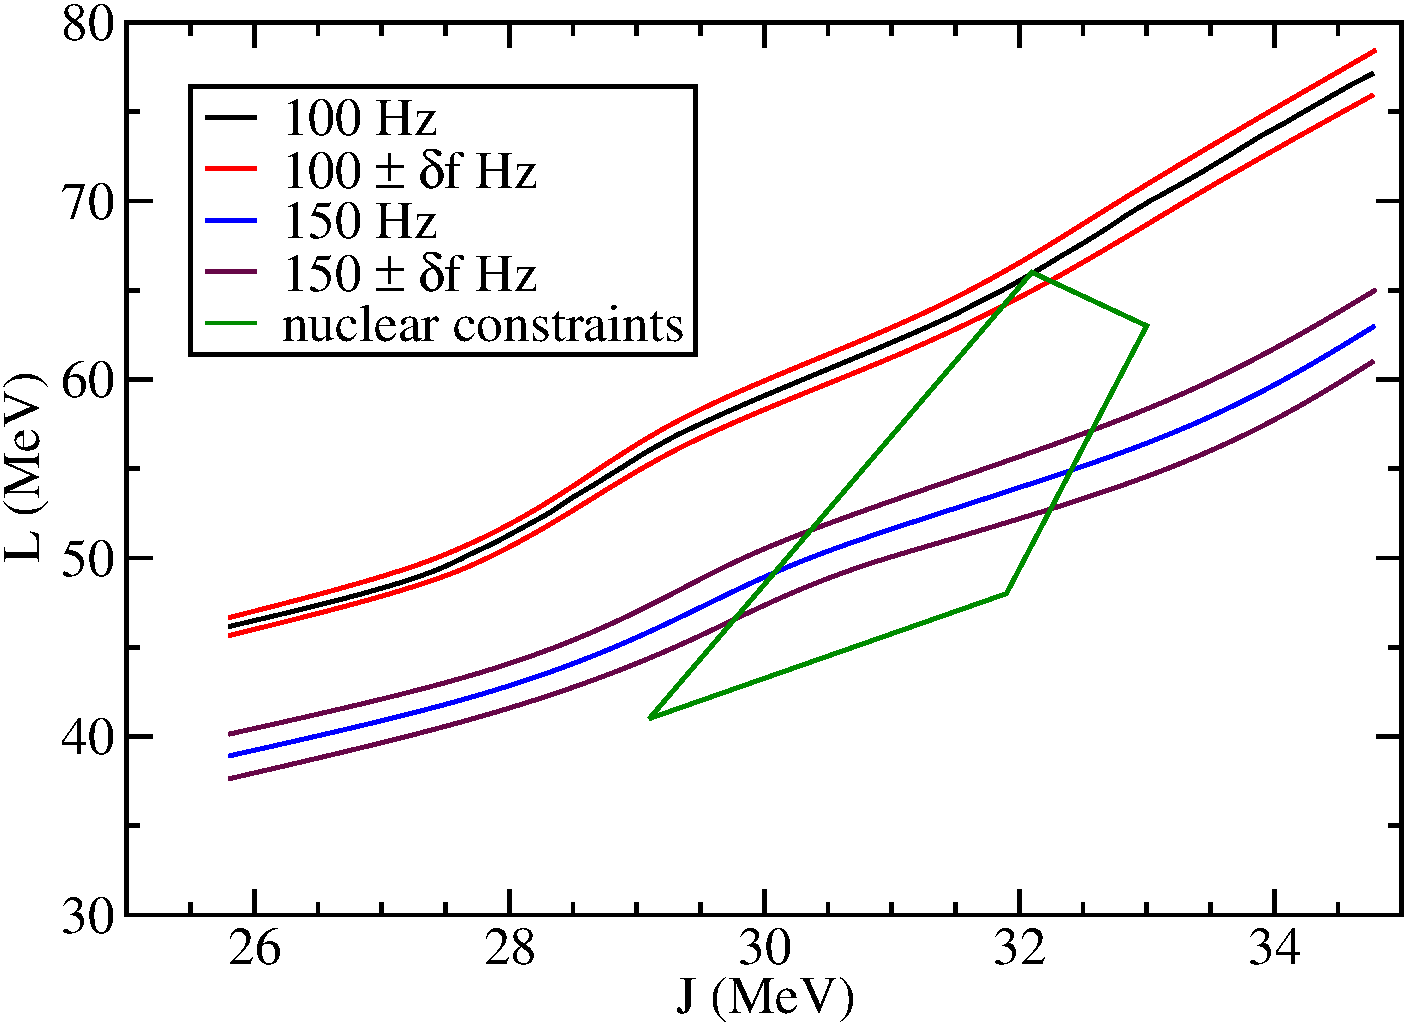
\includegraphics[width=0.45\textwidth,angle=0]{f100_f150_tres_2.pdf}
\caption{Frequency contours in the $J,L$ plane for $K_{\rm sym}$. The black line is for $f=100$ Hz, and the red lines are for $f=100+\delta f$ Hz. The green line is for $f=150$ Hz, and the blue lines are for $f=150+\delta f$ Hz.}
\label{fig:t_res_spread}
\end{figure}

\hspace{\parindent}Figure \ref{fig:M_vs_f} shows that neutron stars with different masses will have different i-mode frequencies, with more massive stars having lower frequencies. This means that, for a specific star, the i-mode frequency will have some degree of uncertainty propagated from the uncertainty in its mass measurement. Figure \ref{fig:vary_mass_contours} shows an example of how this uncertainty affects the $J,L$ constraints. In order to get a reasonable range for the mass uncertainty, the mass values used were taken from the low spin ranges for the stars in GW170817~\cite{abbott2017merger}. The difference between the contours' $L$ values at any given $J$ value is $1-1.5$ MeV. Improved measurements of NS mass would help to reduce this uncertainty, giving us a better constraint.

\begin{figure}
\centering
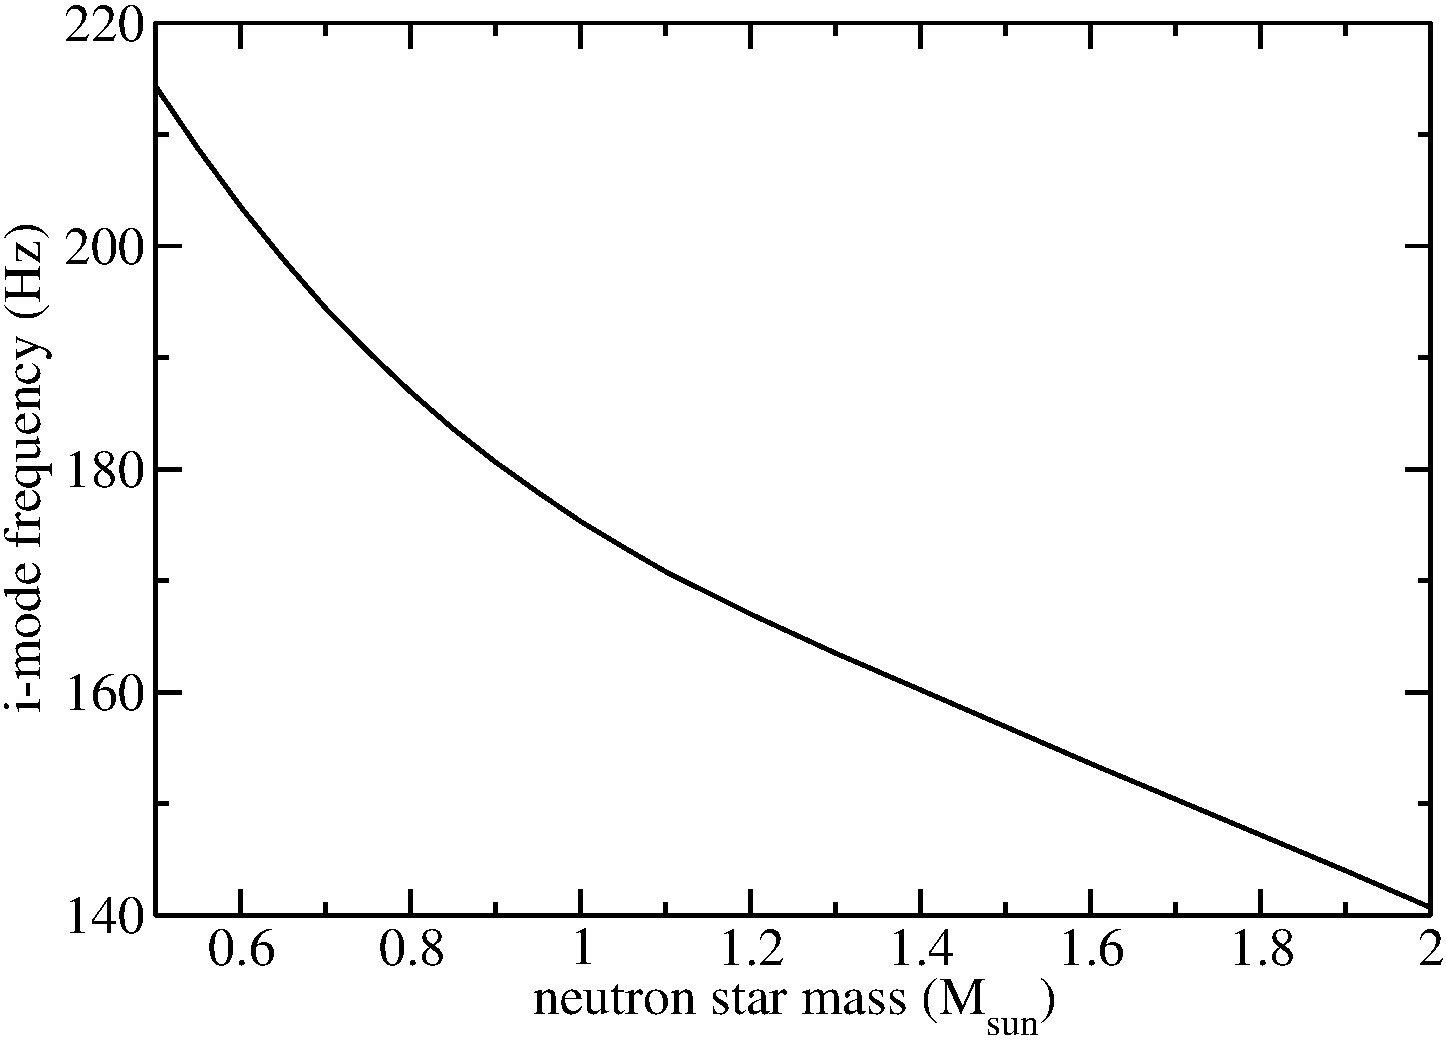
\includegraphics[width=0.45\textwidth,angle=0]{M_vs_f}
\caption{The relationship between NS mass and the i-mode frequency for the sly4 EoS.}
\label{fig:M_vs_f}
\end{figure}

\begin{figure}
\centering
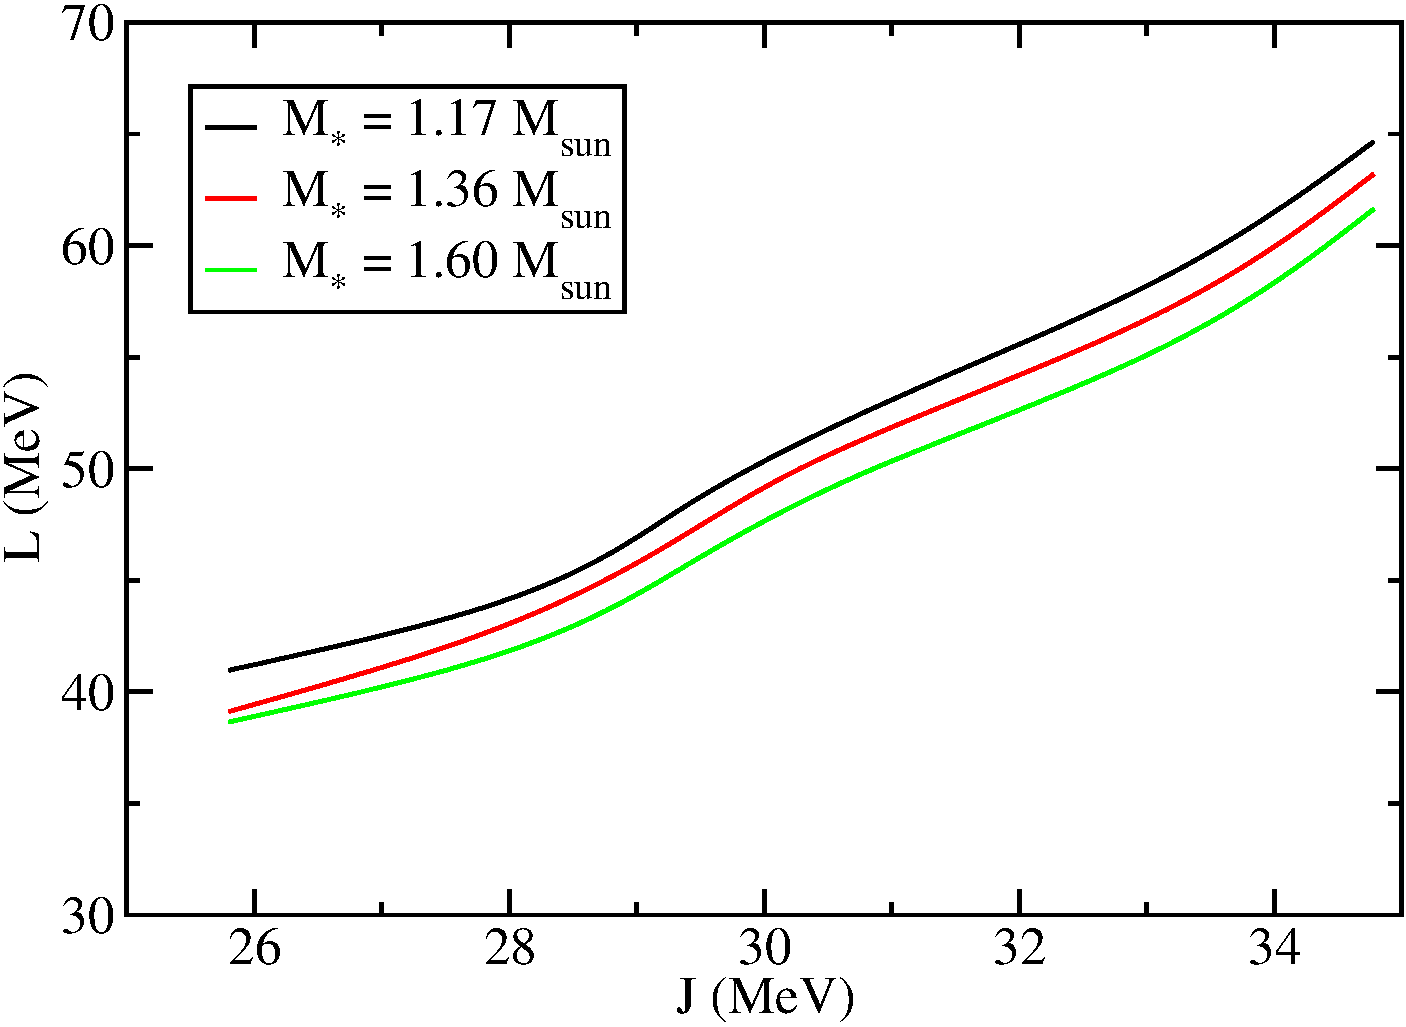
\includegraphics[width=0.45\textwidth,angle=0]{K40_f150_Mcomp.pdf}
\caption{The effect of changing the total NS mass on the symmetry energy parameters that give a frequency of $150$ Hz.}
\label{fig:vary_mass_contours}
\end{figure}





%%%%%%%%%%%%%%%%%%%%%%%%%%%%%%%%%%


\section{Discussion}
%first sentence is repeated. I think it fits better here, so remove/change the earlier occurrence.
\hspace{\parindent}Far from symmetry we would expect higher order symmetry energy parameters ($L$, $K_{\rm sym}$) to have a stronger impact on the frequency than lower order terms ($J$). From figure \ref{fig:freq_contours} this does seem to be the case, with the contours covering a wide range of $J$ values and a smaller range of $L$ values. $K_{\rm sym}$ also has a significant impact on the i-mode frequencies, with the extremes of our $K_{\rm sym}$ range having a difference of $\Delta L\sim 20$ MeV for the same $J$ values. Figure \ref{fig:constraints} shows contours for supposed detections of RSFs at $100$ Hz and $150$ Hz, with the two contours for each frequency showing the upper and lower bounds of the $K_{\rm sym}$ range. $100-150$ Hz was chosen because the precursor occurs roughly half a second before the merger~\cite{zhong2019precursors}, and half a second before the merger, the frequency of GW170817 was $~100-150$ Hz~\cite{abbott2017merger}.

\hspace{\parindent}....................................







\subsection{Comparisons to other constraints}
\hspace{\parindent}There are many different constraints on the symmetry energy parameters that can be found from various properties of nuclei, such as the their masses~\cite{kortelainen2010nuclear} and neutron skins~\cite{chen2010density}. By plotting these constraints together, the symmetry energy parameters $J$ and $L$ can be constrained to a small range of values~\cite{balantekin2014nuclear}. This range is shown in figure \ref{fig:constraints} alongside the contours for RSFs at $100$ Hz and $150 Hz$.
From this figure we see that for an i-mode frequency of $100$ Hz, our constraint has a similar $L$ uncertainty as the nuclear constraints, and so a detection at this value would help provide evidence the currently known constraints on $J$ and $L$. However, for an i-mode frequency of $150$ Hz, the constraint is shifted to significantly lower L values. Therefore a detection of a precursor at $150$ Hz would improve the previous constraints on $J$ and $L$ to approximately $J\approx 30.75\pm 1.65$ MeV, $L\approx 48\pm 7$ MeV. In general, these results prefer $L$ values towards to lower end of the previous constrains. %Cite Lattimer and mention that the dipole polarisability is wrong?
% on the graph of constraints in the J,L plane, my results are similar to those for dipole polarisability
% constrain K using the J,L values?

\begin{figure}
\centering
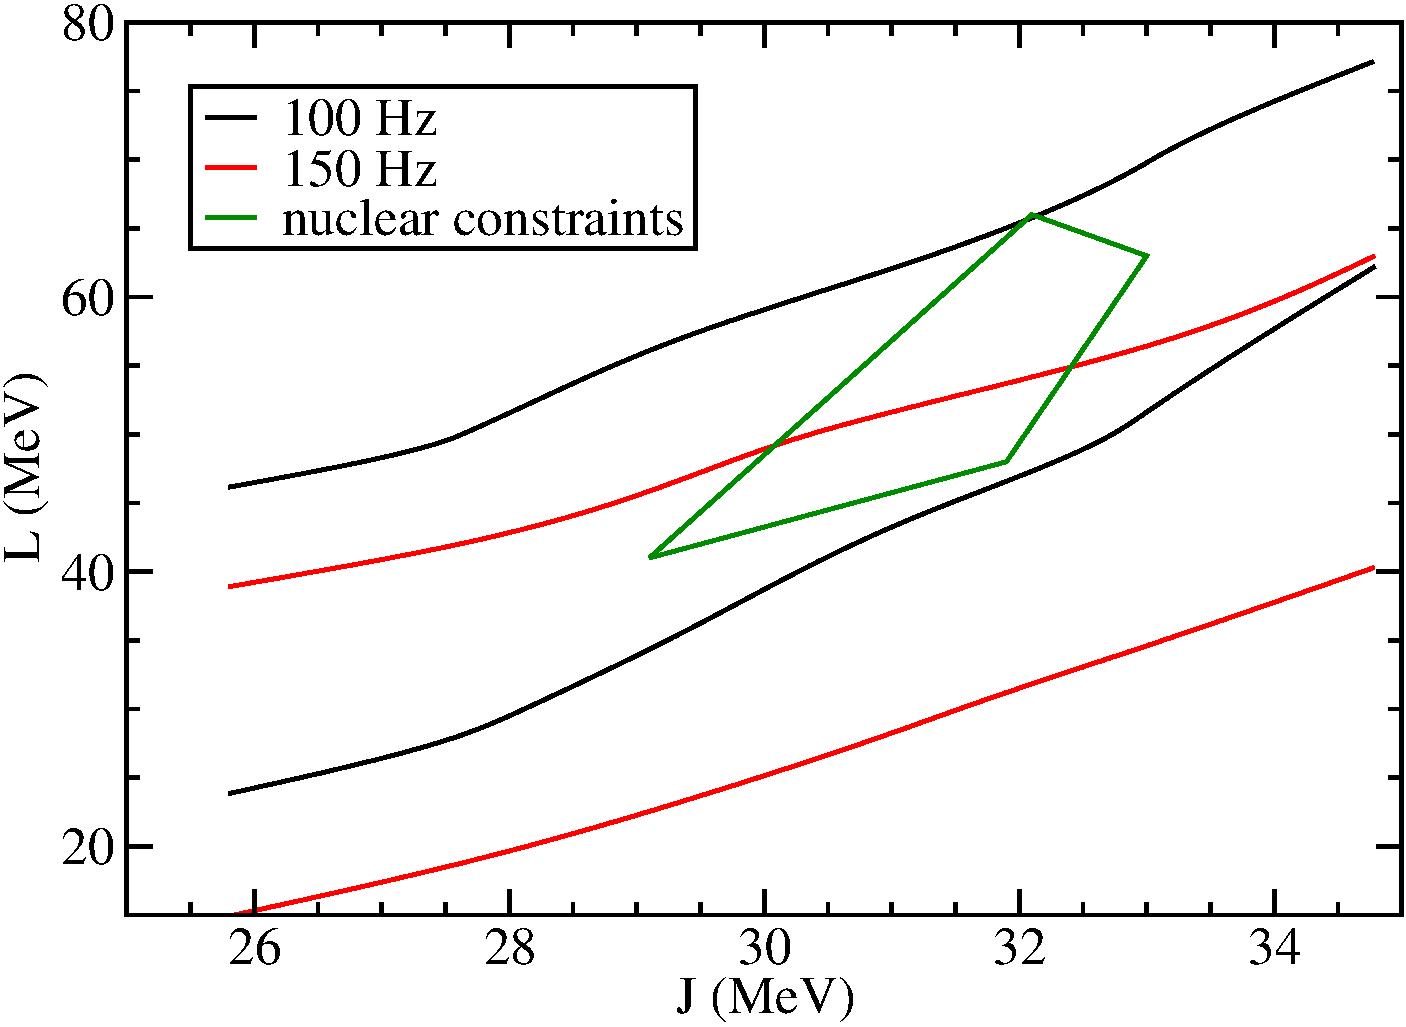
\includegraphics[width=0.45\textwidth,angle=0]{constraints_rough_2}
\caption{<Very rough, replace later> Range in $J,L$ due to the range of $K_{sym}$ values. The upper bound is for K=40 MeV, and the lower bound is for K=-200 MeV.}
\label{fig:constraints}
\end{figure}

\hspace{\parindent}Figure \ref{fig:all_constraints} shows the combination of: the spread in frequency due to $t_{\rm res}$, the range in $L$ due to the uncertainty in stellar mass, and the spread in $L$ due to the range of $K_sym$ values used. This figure shows the most conservative estimate of the $J$, $L$ constraints, with the upper bounds using $M_*=1.17$ M$_{\odot}$, $f\rightarrow f-\delta f$ Hz, and $K_{sym}=40$ MeV and the lower bounds using $M_*=1.36$ M$_{\odot}$, $f\rightarrow f+\delta f$ Hz, and $K_{sym}=-200$ MeV. The ranges shown in this figure are slightly different to figure \ref{fig:constraints}, but the main uncertainty is the $K_{sym}$ range.




%figure that combines all uncertainties (K_sym value, NS mass, t_res range), explain this one in text.
\begin{figure}
\centering
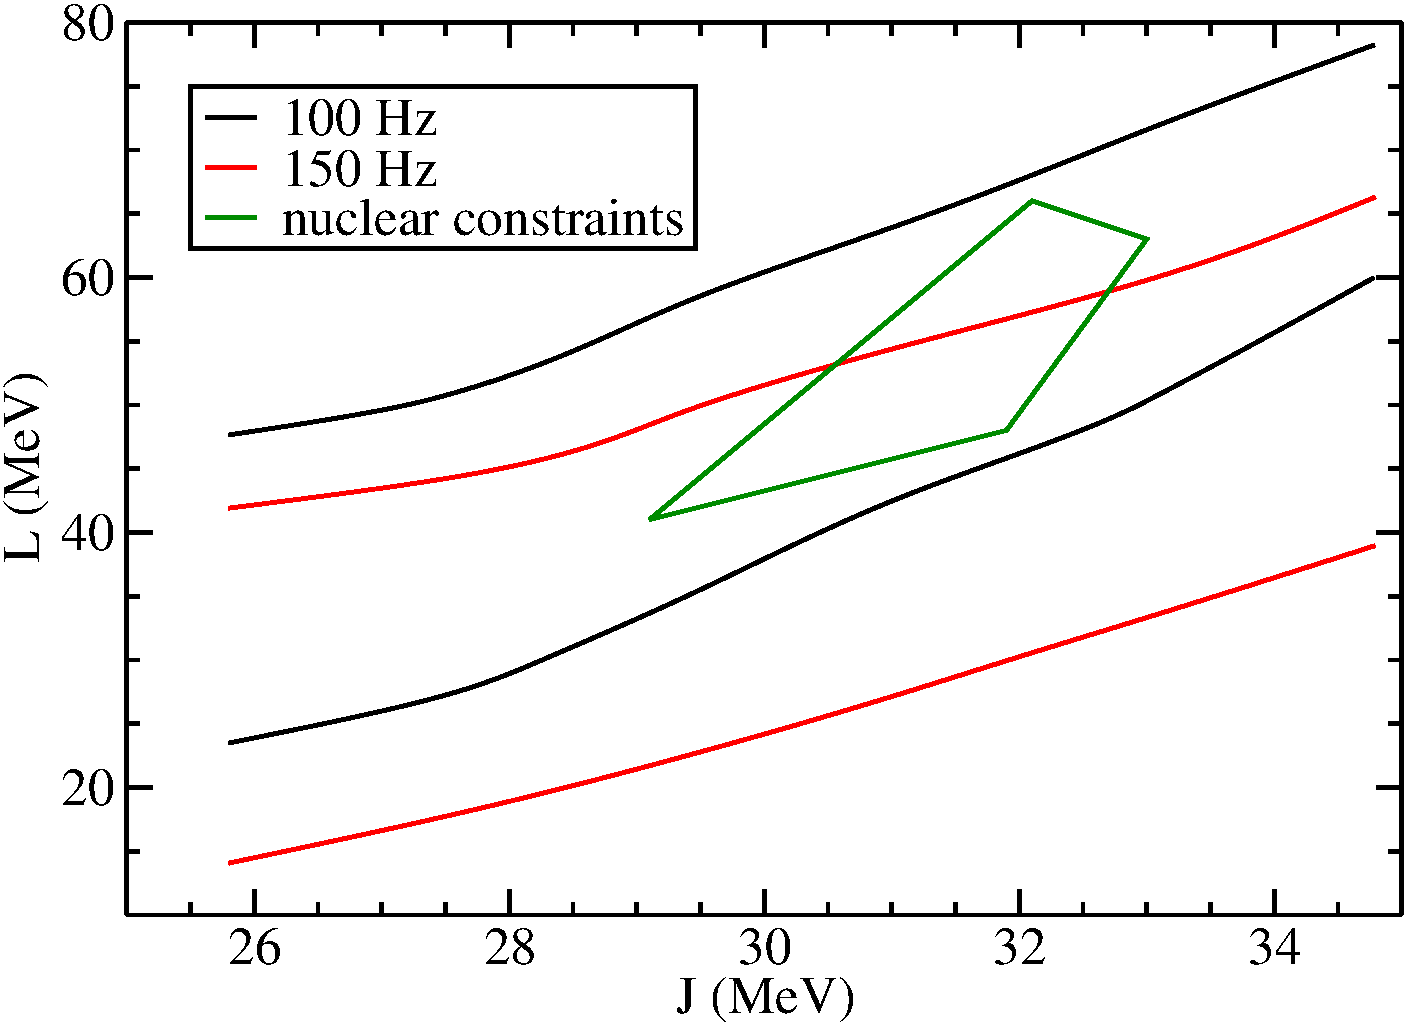
\includegraphics[width=0.45\textwidth,angle=0]{K_M_tres_ranges.pdf}
\caption{<Very rough, replace later> Combines the ranges from figures \ref{fig:t_res_spread}, \ref{fig:vary_mass_contours}, and \ref{fig:constraints}.} %Upper bound is K=40 MeV, lower bound is K=-200 MeV.
\label{fig:all_constraints}
\end{figure}















%%%%%%%%%%%%%%%%%%%% REFERENCES %%%%%%%%%%%%%%%%%%

% The best way to enter references is to use BibTeX:

\bibliographystyle{mnras}
\bibliography{example} % if your bibtex file is called example.bib


% Alternatively you could enter them by hand, like this:
% This method is tedious and prone to error if you have lots of references
%\begin{thebibliography}{99}
%\bibitem[\protect\citeauthoryear{Author}{2012}]{Author2012}
%Author A.~N., 2013, Journal of Improbable Astronomy, 1, 1
%\bibitem[\protect\citeauthoryear{Others}{2013}]{Others2013}
%Others S., 2012, Journal of Interesting Stuff, 17, 198
%\end{thebibliography}

%%%%%%%%%%%%%%%%%%%%%%%%%%%%%%%%%%%%%%%%%%%%%%%%%%

%%%%%%%%%%%%%%%%% APPENDICES %%%%%%%%%%%%%%%%%%%%%

\appendix

\section{Some extra material}

If you want to present additional material which would interrupt the flow of the main paper,
it can be placed in an Appendix which appears after the list of references.

%%%%%%%%%%%%%%%%%%%%%%%%%%%%%%%%%%%%%%%%%%%%%%%%%%


% Don't change these lines
\bsp	% typesetting comment
\label{lastpage}
\end{document}

% End of mnras_template.tex
